\documentclass[a4paper,twoside]{article}
\usepackage[T1]{fontenc}
\usepackage[bahasa]{babel}
\usepackage{graphicx}
\usepackage{graphics}
\usepackage{float}
\usepackage[cm]{fullpage}
\pagestyle{myheadings}
\usepackage{etoolbox}
\usepackage{setspace} 
\usepackage{lipsum} 
\usepackage{url}
\setlength{\headsep}{30pt}
\usepackage[inner=2cm,outer=2.5cm,top=2.5cm,bottom=2cm]{geometry} %margin
% \pagestyle{empty}

\makeatletter
\renewcommand{\@maketitle} {\begin{center} {\LARGE \textbf{ \textsc{\@title}} \par} \bigskip {\large \textbf{\textsc{\@author}} }\end{center} }
\renewcommand{\thispagestyle}[1]{}
\markright{\textbf{\textsc{Laporan Perkembangan Pengerjaan Skripsi\textemdash Sem. Ganjil 2015/2016}}}

\onehalfspacing
 
\begin{document}

\title{\@judultopik}
\author{\nama \textendash \@npm} 

%ISILAH DATA DATA BERIKUT INI:
\newcommand{\nama}{Herfan Heryandi}
\newcommand{\@npm}{2012730012}
\newcommand{\tanggal}{03/10/2015} %Tanggal pembuatan dokumen
\newcommand{\@judultopik}{IT STUDENT PORTAL: PEMANFAATAN \textit{WEB SCRAPING} UNTUK KUSTOMISASI PORTAL AKADEMIK MAHASISWA} % Judul/topik anda
\newcommand{\kodetopik}{PAS3904}
\newcommand{\jumpemb}{1} % Jumlah pembimbing, 1 atau 2
\newcommand{\pembA}{Pascal Alfadian}
\newcommand{\pembB}{-}
\newcommand{\semesterPertama}{39 - Ganjil 15/16} % semester pertama kali topik diambil, angka 1 dimulai dari sem Ganjil 96/97
\newcommand{\lamaSkripsi}{1} % Jumlah semester untuk mengerjakan skripsi s.d. dokumen ini dibuat
\newcommand{\kulPertama}{Skripsi 1} % Kuliah dimana topik ini diambil pertama kali
\newcommand{\tipePR}{B} % tipe progress report :
% A : dokumen pendukung untuk pengambilan ke-2 di Skripsi 1
% B : dokumen untuk reviewer pada presentasi dan review Skripsi 1
% C : dokumen pendukung untuk pengambilan ke-2 di Skripsi 2

% Dokumen hasil template ini harus dicetak bolak-balik !!!!

\maketitle

\pagenumbering{arabic}

\section{Data Skripsi} %TIDAK PERLU MENGUBAH BAGIAN INI !!!
Pembimbing utama/tunggal: {\bf \pembA}\\
Pembimbing pendamping: {\bf \pembB}\\
Kode Topik : {\bf \kodetopik}\\
Topik ini sudah dikerjakan selama : {\bf \lamaSkripsi} semester\\
Pengambilan pertama kali topik ini pada : Semester {\bf \semesterPertama} \\
Pengambilan pertama kali topik ini di kuliah : {\bf \kulPertama} \\
Tipe Laporan : {\bf \tipePR} -
\ifdefstring{\tipePR}{A}{
			Dokumen pendukung untuk {\BF pengambilan ke-2 di Skripsi 1} }
		{
		\ifdefstring{\tipePR}{B} {
				Dokumen untuk reviewer pada presentasi dan {\bf review Skripsi 1}}
			{	Dokumen pendukung untuk {\bf pengambilan ke-2 di Skripsi 2}}
		}

\section{Detail Perkembangan Pengerjaan Skripsi}
Detail bagian pekerjaan skripsi sesuai dengan rencana kerja/laporan perkembangan terakhir :
	\begin{enumerate}
		%NOMOR 1%
		\item Melakukan studi mengenai \textit{library} jsoup, Chrome DevTools, Play Framework, SIA Models, dan CSS \textit{Selector}.\\
		{\bf status :} Ada sejak rencana kerja skripsi kecuali SIA Models dan CSS \textit{Selector}.\\
		{\bf hasil :} \\

		
		%NOMOR 2%
		\item Melakukan wawancara kepada mahasiswa Program Studi Teknik Informatika untuk mendapatkan informasi
penggunaan Portal Akademik Mahasiswa dan fitur-fitur yang diinginkan.\\
		{\bf status :} Ada sejak rencana kerja skripsi.\\
		{\bf hasil :} Wawancara sudah dilakukan kepada 18 mahasiswa Program Studi Teknik Informatika. Bukti-bukti wawancara dapat dilihat pada \url{https://github.com/herfanheryandi/Skripsi/tree/master/draft/Interview/}. Dari hasil wawancara tersebut, diperoleh fitur-fitur yang diinginkan mahasiswa antara lain:
		\begin{enumerate}
	\item Prasyarat mata kuliah\\
	Mahasiswa bisa memeriksa prasyarat mata kuliah saat FRS sehingga tidak terjadi kesalahan pengambilan mata kuliah. Prasyarat mata kuliah yang ditampilkan di Portal Akademik Mahasiswa kurang akurat. Selain itu, dari 18 mahasiswa yang diwawancara, hanya ada satu mahasiswa yang mengetahui bahwa Portal Akademik Mahasiswa memiliki fitur prasyarat. Prasyarat mata kuliah untuk Program Studi Teknik Informatika juga tersedia di \url{http://tinyurl.com/lionov}, namun mahasiswa merasa kurang praktis karena harus memeriksa secara manual. Mahasiswa menginginkan agar fitur ini bisa dibuat untuk mempermudah FRS.
	\item Ringkasan data akademik\\
	Ringkasan data akademik menampilkan data mengenai mata kuliah wajib, pilihan, dan pilihan wajib yang sudah lulus, mata kuliah wajib yang belum lulus, dan sisa SKS untuk mencapai kelulusan. Mahasiswa menginginkan fitur ini dibuat untuk membantu mahasiswa dalam mengatur perkuliahannya.
	\item Perubahan IPS dan IPK berdasarkan riwayat nilai\\
	Dalam Portal Akademik Mahasiswa, nilai pertama kali muncul dalam riwayat nilai. Riwayat IP tidak berubah secara otomatis saat seluruh nilai di riwayat nilai sudah muncul. Mahasiswa menginginkan agar IPS dan IPK dapat berubah secara otomatis saat nilai muncul.
	\item Jadwal kuliah yang tersusun\\
	Tampilan jadwal kuliah dalam Portal Akademik Mahasiswa tidak terurut berdasarkan hari seperti pada gambar \ref{fig:3_jadwal_portal} sehingga perlu direkapitulasi lagi. Mahasiswa menginginkan agar tampilan jadwal tersusun dan dalam bentuk seperti gambar \ref{fig:3_jadwal_rekap}.
		\begin{figure}[H]
			\centering
			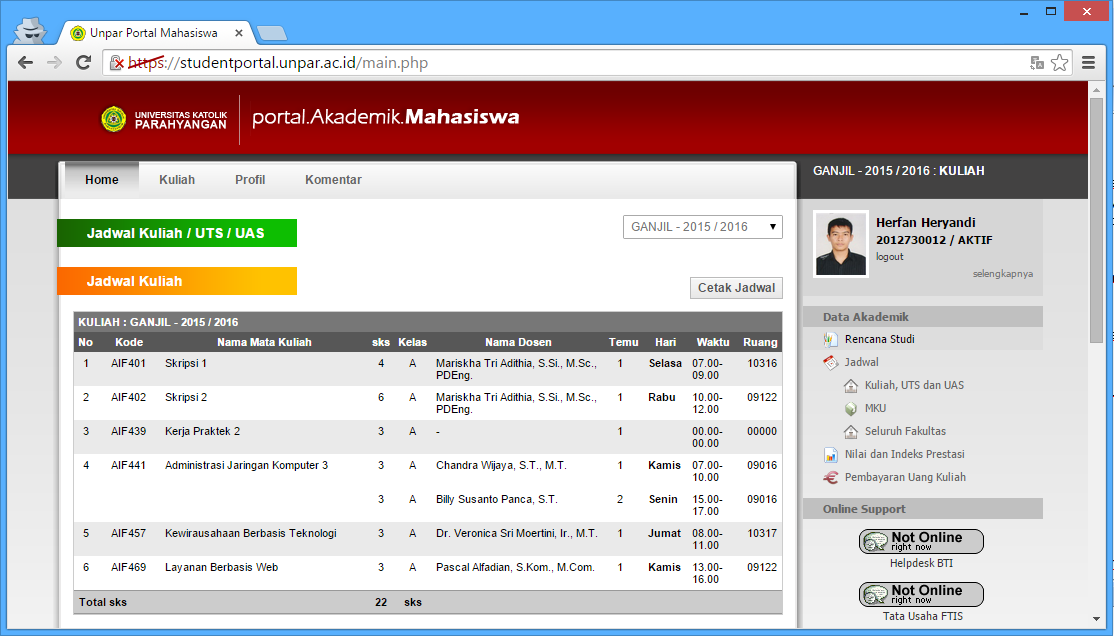
\includegraphics[scale=0.5]{Gambar/jadwal-portal}
			\caption{Tampilan Jadwal pada Portal Akademik Mahasiswa} 
			\label{fig:3_jadwal_portal}
		\end{figure}
		
		\begin{figure}[H]
			\centering
			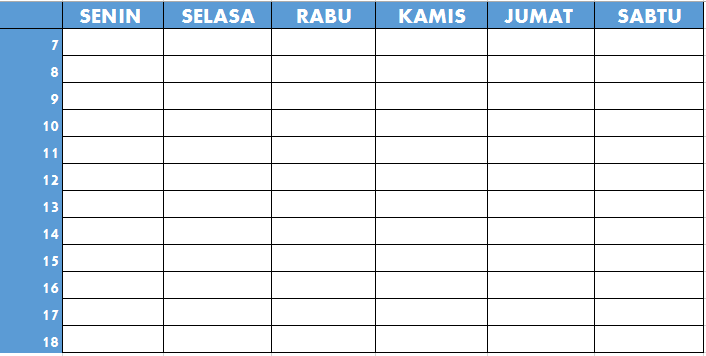
\includegraphics[scale=0.5]{Gambar/jadwal-rekap}
			\caption{Tampilan Jadwal yang Diinginkan Mahasiswa} 
			\label{fig:3_jadwal_rekap}
		\end{figure}
		
	\item Kalender akademik\\
	Kalender akademik merupakan salah satu fitur pada Portal Akademik Mahasiswa namun sekarang fitur tersebut sudah tidak ada lagi. Mahasiswa menginginkan fitur kalender akademik kembali untuk mengetahui tanggal-tanggal penting pada perkuliahan. 
	\item Rincian pembayaran\\
	Tagihan pada Portal Akademik Mahasiswa tidak mencantumkan batas akhir pembayaran dan rincian nominal tagihan. Mahasiswa menginginkan rincian pembayaran agar tidak terlambat membayar uang kuliah dan dapat mengetahui rincian nominal tagihan.
	\item Rincian mata kuliah\\
	Setiap mata kuliah yang dibuka memiliki rincian seperti deskripsi mata kuliah dan jenis mata kuliah yaitu apakah mata kuliah tersebut wajib, pilihan, atau pilihan wajib. Mahasiswa menginginkan fitur ini agar dapat mengetahui mata kuliah apa yang akan dipelajari.
	\item Tampilan situs web sama di sistem operasi manapun\\
	Jika tidak menggunakan sistem operasi Windows seperti Linux dan Mac, saat mengakses Portal Akademik Mahasiswa melalui \url{https://studentportal.unpar.ac.id/}, maka mahasiswa akan diarahkan ke \url{https://m.studentportal.unpar.ac.id/} yaitu Portal Akademik Mahasiswa dengan tampilan \textit{mobile} (Gambar \ref{fig:3_pam_mobile}). Tampilan ini tidak memiliki fitur selengkap Portal Akademik Mahasiswa, hanya memiliki fitur pengumunan kuliah, jadwal kuliah, UTS, dan UAS, nilai, IP, dan tagihan. Selain itu, tampilan \textit{mobile} pada telepon seluler akan terlihat sangat kecil sehingga tidak sulit untuk memilih menu. Mahasiswa menginginkan fitur ini agar IT Student Portal dapat diakses di sistem operasi manapun tanpa perubahan tampilan.
	\begin{figure}[H]
			\centering
			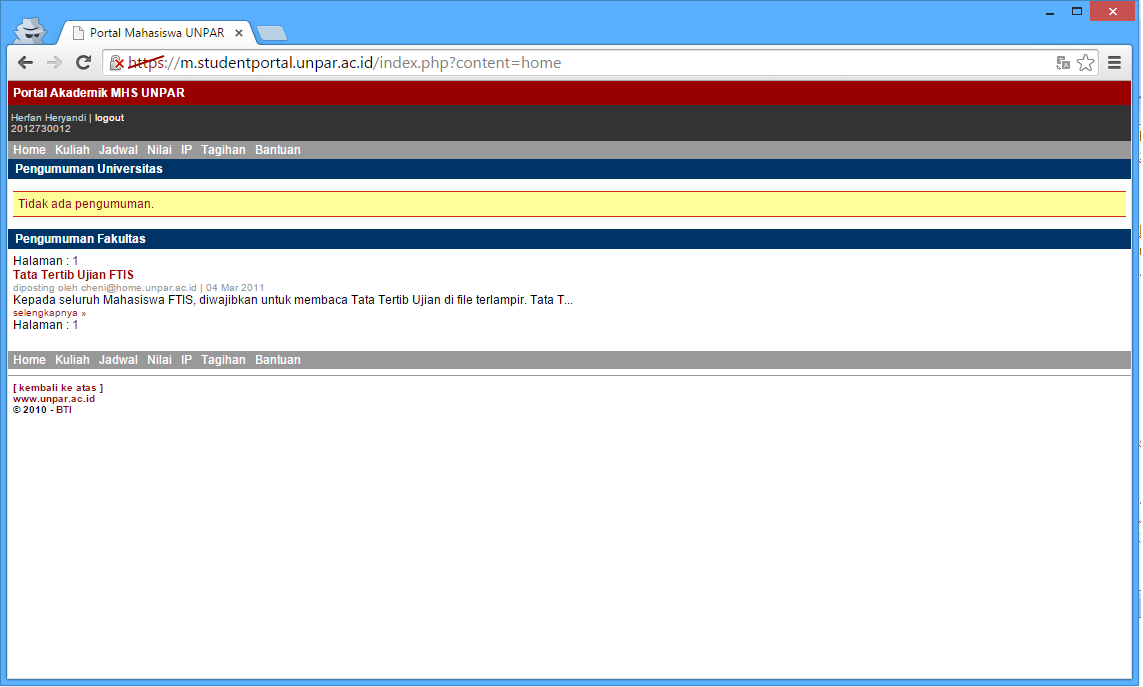
\includegraphics[scale=0.5]{Gambar/pam-mobile}
			\caption{Tampilan \textit{Mobile} Portal Akademik Mahasiswa} 
			\label{fig:3_pam_mobile}
		\end{figure}
	\item Kontak dosen\\
	Kontak dosen berisi informasi email setiap dosen sehingga dapat mempermudah mahasiswa untuk menghubungi dosen. Mahasiswa juga dapat mengirim email secara langsung melalui Portal Akademik Mahasiswa.
	\item Pohon kurikulum\\
	Mahasiswa munginnginkan agar dapat melihat pohon kurikulum Program Studi Teknik Informatika dalam Portal Akademik Mahasiswa.
	\item Pemberitahuan\\
	Mahasiswa menginginkan Portal Akademik Mahasiswa menampilkan pemberitahuan berupa \textit{pop up} mengenai pengumuman terkini.
	\item \textit{Chatting}\\
	Mahasiswa menginginkan agar dapat berkomunikasi dengan sesama pengguna Portal Akademik Mahasiswa melalui \textit{chat}.
	\item Unggah \textit{Curriculum Vitae}
	Mahasiswa menginginkan agar dapat mengunggah data mengenai kegiatan dan keaktifan di universitas agar dapat digunakan oleh perusahaan untuk mencari mahasiswa dengan kriteria tertentu misalnya untuk kepentingan magang dan beasiswa.
\end{enumerate}
		
		%NOMOR 3%
		\item Menganalisis Portal Akademik Mahasiswa dan Perancangan IT Student Portal.\\
		{\bf status :} Ada sejak rencana kerja skripsi, kecuali Analisis Perancangan IT Student Portal.\\
		{\bf hasil :} Portal Akademik Mahasiswa sudah berhasil dianalisis. untuk memenuhi fitur IT Student Portal.

		\item Mengimplementasikan \textit{web scraping} menggunakan \textit{library} jsoup.\\
		{\bf status :} Ada sejak rencana kerja skripsi.\\
		{\bf hasil :} -
		\item Membangun perangkat lunak IT Student Portal.\\
		{\bf status :} Ada sejak rencana kerja skripsi.\\
		{\bf hasil :} -

		\item Melakukan eksperimen dan pengujian\\
		{\bf status :} Ada sejak rencana kerja skripsi.\\
		{\bf hasil :} -

		\item Menulis dokumen skripsi\\
		{\bf status :} Ada sejak rencana kerja skripsi.\\
		{\bf hasil :} Dokumen skripsi sudah ditulis hingga bab 3.

	\end{enumerate}

\section{Pencapaian Rencana Kerja}
Persentase penyelesaian skripsi sampai dengan dokumen ini dibuat dapat dilihat pada tabel berikut :

\begin{center}
  \begin{tabular}{ | c | c | c | c | l | c |}
    \hline
    1*  & 2*(\%) & 3*(\%) & 4*(\%) &5* &6*(\%)\\ \hline \hline
   1   & 14  & 14  &  &  & 13\\ \hline
    2   & 14 & 14  &   &  & 14\\ \hline
    3   & 14  & 14  &  &  & 13\\ \hline
    4   & 14  &   &  14 &  & \\ \hline
    5   & 14  &   & 14 &  & \\ \hline
    6   & 14 &   & 14  &  & \\ \hline
    7   & 16  & 8  & 8 &  {\footnotesize bab 1, bab 2, dan bab 3 di S1} & 7\\ \hline
    Total  & 100  & 50  & 50 &  & 47\\ \hline
                          \end{tabular}										
\end{center}

Keterangan (*)\\
1 : Bagian pengerjaan Skripsi (nomor disesuaikan dengan detail pengerjaan di bagian 5)\\
2 : Persentase total \\
3 : Persentase yang akan diselesaikan di Skripsi 1 \\
4 : Persentase yang akan diselesaikan di Skripsi 2 \\
5 : Penjelasan singkat apa yang dilakukan di S1 (Skripsi 1) atau S2 (skripsi 2)\\
6 : Persentase yang sudah diselesaikan sampai saat ini 

%\section{Kendala yang dihadapi}
%TULISKAN BAGIAN INI JIKA DOKUMEN ANDA TIPE A ATAU C
%Kendala - kendala yang dihadapi selama mengerjakan skripsi :
%\begin{itemize}
%	\item Terlalu banyak melakukan prokratinasi
%	\item Mengalami kesulitan dalam instalasi Play Framework
%	\item Kurang familiar dengan pemrograman Play Framework
%\end{itemize}

\vspace{1cm}
\centering Bandung, \tanggal\\
\vspace{2cm} \nama \\ 
\vspace{1cm}

Menyetujui, \\
\ifdefstring{\jumpemb}{2}{
\vspace{1.5cm}
\begin{centering} Menyetujui,\\ \end{centering} \vspace{0.75cm}
\begin{minipage}[b]{0.45\linewidth}
% \centering Bandung, \makebox[0.5cm]{\hrulefill}/\makebox[0.5cm]{\hrulefill}/2013 \\
\vspace{2cm} Nama: \pembA \\ Pembimbing Utama
\end{minipage} \hspace{0.5cm}
\begin{minipage}[b]{0.45\linewidth}
% \centering Bandung, \makebox[0.5cm]{\hrulefill}/\makebox[0.5cm]{\hrulefill}/2013\\
\vspace{2cm} Nama: \pemB \\ Pembimbing Pendamping
\end{minipage}
\vspace{0.3cm}
}{
% \centering Bandung, \makebox[0.5cm]{\hrulefill}/\makebox[0.5cm]{\hrulefill}/2013\\
\vspace{2cm} Nama: \pembA \\ Pembimbing Tunggal
}
`
\end{document}

